\documentclass[fleqn]{exam}

\usepackage{fullpage}
\usepackage{enumerate}
% \usepackage{siunitx} 
\usepackage{unitsdef} 
\usepackage{graphicx}
\usepackage[fleqn]{mathtools}
\usepackage{cancel}
\usepackage{polynom}
\usepackage{float}
\usepackage{mdwlist}
\usepackage{booktabs}
\usepackage{cancel}
\usepackage{polynom}
\usepackage{caption}

\setlength{\mathindent}{.5 cm}


\everymath{\displaystyle}

% \begin{figure}[H]
%   \centering
%   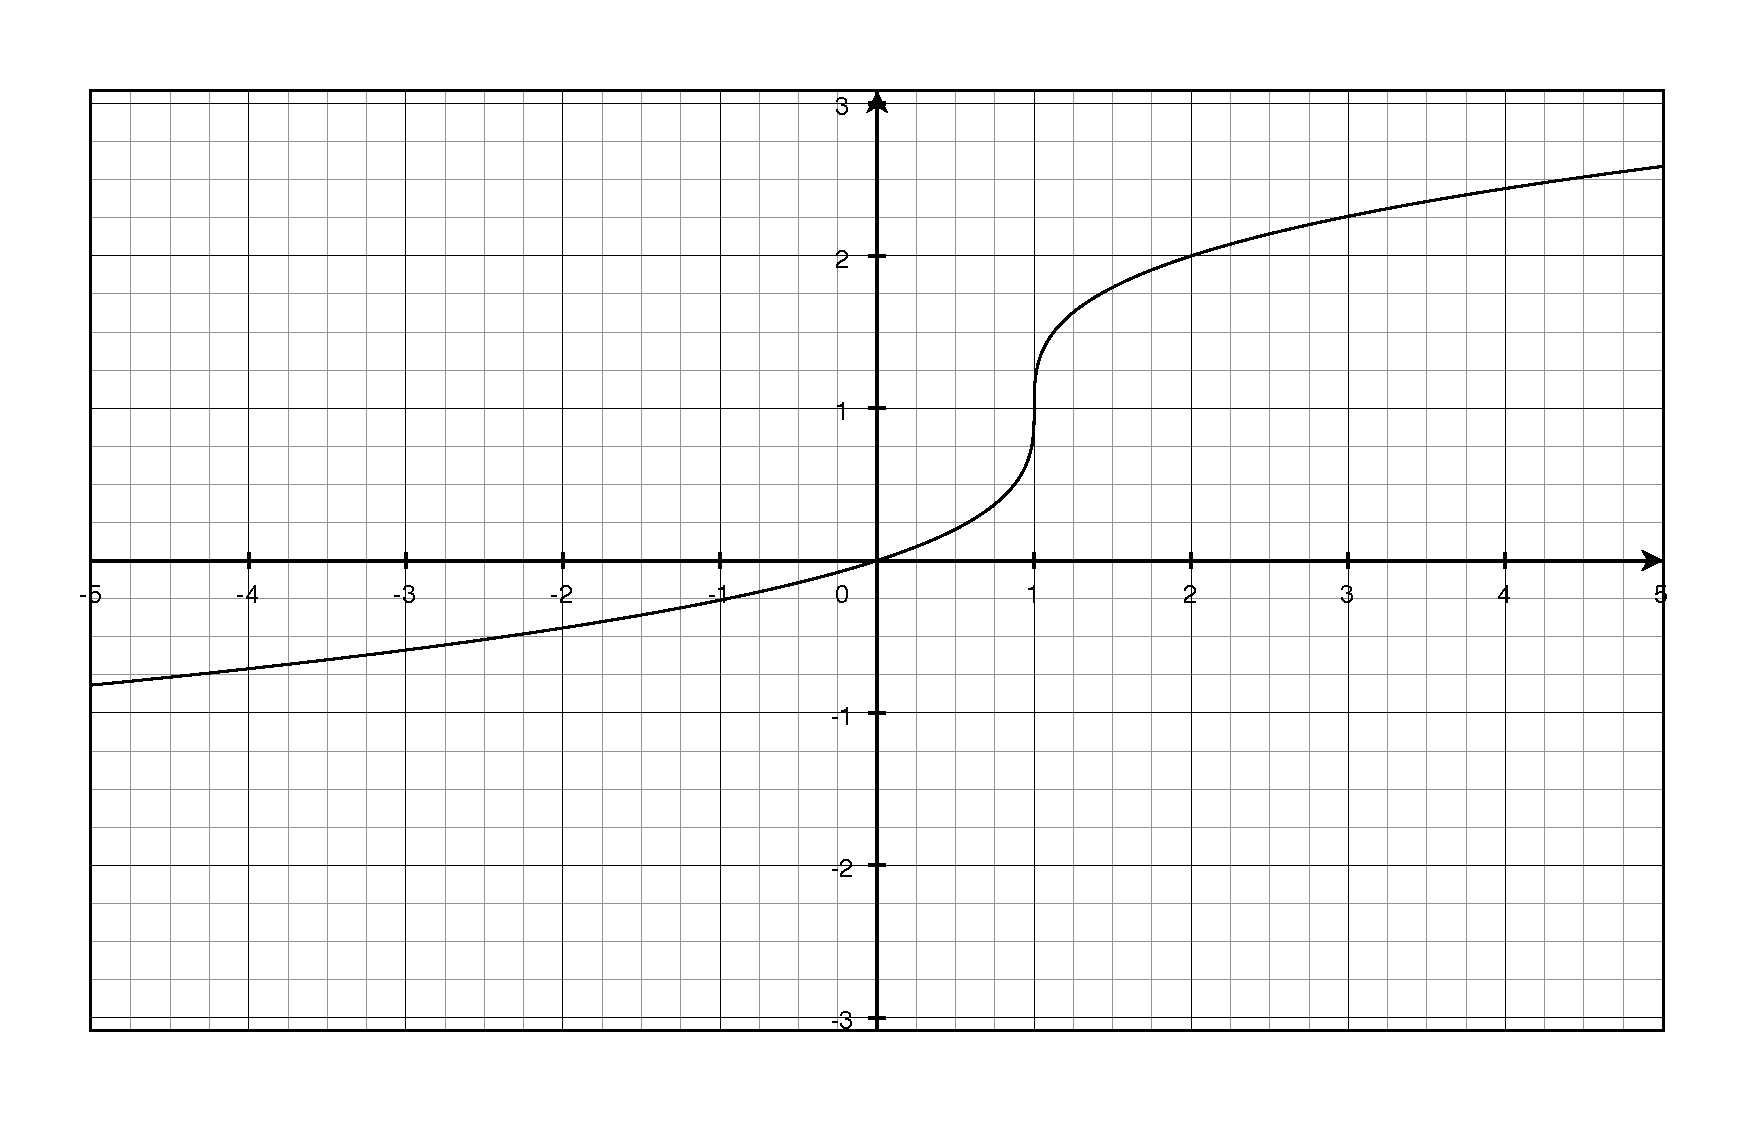
\includegraphics[scale=.3]{question7.eps}
%   \caption*{Question 7}
% \end{figure}

% \begin{tabular}{cc}
% \toprule
% period & amplitude \\
% \midrule
%   $\pi$ & $2$ \\
% \bottomrule
% \end{tabular}

\newunit{\inch}{in}
\newunit{\mile}{mile}
\newunit{\foot}{ft}
\newunit{\knot}{knot}

\printanswers

\ifprintanswers 
\usepackage{2in1, lscape} 
\fi

\title{Math 263a \\ Homework 10}
\date{March 28, 2012}

\begin{document}

\maketitle

\section{Homework}

\begin{itemize*}
  \item Read Section 3.9
  \item pp. 160-162: 2-3, 5-9, 13-17, 19, 21-22, 25
\end{itemize*}

\section{Extra Credit}
Page 162, problems 28 and 29

\begin{description}
\pagebreak

\item[28]
If you draw a picture of the situation and call $x$ the length of the shadow and $y$ the height of the ball, when the
ball is below 48 feet, it creates two similar triangles.  One of the triangles has the street light as one side and the
other triangle has the ball height on the corresponding side.

\begin{align*}
  \frac{y}{x} &= \frac{48}{x + 10} \\
  xy + 10y &= 48x \\
  x \frac{dy}{dt} + y \frac{dx}{dt} + 10 \frac{dy}{dt} &= 48 \frac{dx}{dt} \\
  \frac{dx}{dt} &= \frac{dy}{dt} \cdot \frac{x + 10}{48 - x} \\
\end{align*}

If we make the ground 0, $y = 64 - 16t^2$, $\frac{dy}{dt} = -32t$.  To find a value for $\frac{dy}{dt}$, we need to know how long it takes the
ball to go 64 feet:
\begin{align*}
  16t^2 &= 64 \\
  t &= 2 \\
\end{align*}

Now we have everything we need to find the speed of the shadow when $x$ and $y$ are 0 and $\frac{dy}{dt} = -64$:
\begin{align*}
  \frac{dx}{dt} &= -64 \cdot \frac{10}{48} \\
  &\approx - 13.33 \foot / \second \\
\end{align*}

\pagebreak

\item[29]
First come up with a general expression for either person's shadow growth:

If $h$ is the height of the person, $s$ is the length of the shadow, and $x$ is the distance of the person from the light:
\begin{align*}
  \frac{h}{s} &= \frac{20}{x + s} \\
  20s &= hx + hs \\
  20s \frac{ds}{dt} &= \frac{dx}{dt} \left( \frac{h}{20 - h} \right) \\
\end{align*}

This is the rate of growth of the shadow.  The movement of the tip should also have the speed of the walking added to
it.

For the girl:
\[
  \frac{ds}{dt} = 4 \left( \frac{5}{15} \right) = \frac{4}{3}
\]
So here shadow moves at $\frac{16}{3} \foot / \second$.

For the boy:
\[
  \frac{ds}{dt} = 4 \left( \frac{3}{17} \right) = \frac{12}{17}
\]
So here shadow moves at $\frac{80}{17} \foot / \second$.

Now we need to figure out whose shadow is visible.  The transition occurs when the tops of the heads and the light all
line up.  This happens when the three points: $(0, 20)$, $(x_{girl}, 5)$, and $(x_{girl} + 4, 3)$ are all on the same
line. 
\begin{align*}
  \frac{20 - 5}{-x_{girl}} &= \frac{20 - 3}{-x_{girl} - 4} \\
  x_{girl} &= 30 \foot \\
\end{align*}

\begin{itemize}
\item When the girl is more than 30 feet from the pole, her shadow determines the end point and the shadow tip moves at
$\frac{16}{3} \foot / \second$.

\item When the girl is less than 30 feet from the pole, the boy's shadow determines the end point and the shadow tip moves at
$\frac{80}{17} \foot / \second$.

\end{itemize}

 

\end{description}

\ifprintanswers

\section{Section 3.9}

\begin{description}
\item[2]
\begin{align*}
  V &= \frac{4}{3} \pi r^3  \\
  \frac{dV}{dt} &= 4 \pi r^2 \frac{dr}{dt}  \\
  \frac{dr}{dt} &= \frac{1}{4 \pi r^2} \frac{dV}{dt} \\
  \\
  \frac{dr}{dt} &= \frac{1}{4 \pi \cdot 3^2} \cdot 3^3 \\
                &= \frac{1}{12 \pi} \inch / \second \\
                &\approx 0.027 \inch / \second \\
\end{align*}

\item[3]
After 45 seconds, the plane is 5 miles away, so $x= 5$ and $r = \sqrt{26}$ at the time we are interested in.
 
\begin{align*}
  r^2 &= x^2 + 1  \\
  2 r \frac{dr}{dt} &= 2x \frac{dx}{dt} \\
  \frac{dr}{dt} &= \frac{x}{r} \frac{dx}{dt}
  \\
  \frac{dr}{dt} &= \frac{5}{\sqrt{26}} \cdot 400 \mile / \hour \\
                &\approx  392 \mile / \hour \\
\end{align*}

\pagebreak

\item[5]
If we make 1:00 the time when t is 0, the positions are given by:
\begin{align*}
  x &= 300(t + 1) \\
  y &= 400 t \\
  r &= \sqrt{x^2 + y^2} \\
\end{align*}
\begin{align*}
  r^2 &= x^2 + y^2 \\
  \frac{dr}{dt} &= \frac{x}{r} \cdot \frac{dx}{dt} + \frac{y}{r} \cdot \frac{dy}{dt} \\
  \\
  \frac{dr}{dt} &\approx \frac{600}{721} \cdot 300 + \frac{400}{721} \cdot 400  \\
  &\approx 471 \mile / \hour \\
\end{align*}

\item[6]
\begin{align*}
  r^2 &= x^2 + 10^2 \\
  2 r \frac{dr}{dt} &= 2x \frac{dx}{dt} \\
  \frac{dx}{dt} &= \frac{r}{x} \frac{dr}{dt} \\
  \\
  \frac{dx}{dt} &= \frac{25}{\sqrt{25^2 - 10^2}} \cdot (-2) \foot / \second \\
  &\approx -2.18 \foot / \second \\
\end{align*}

\item[7]
\begin{align*}
  y^2 &= 20^2 - x^2 \\
  \frac{dy}{dt} &= -\frac{x}{y} \frac{dx}{dt} \\
  \\
  \frac{dy}{dt} &= -\frac{5}{\sqrt{20^2 - 5^2}} \cdot 1 \foot / \second \\
  &\approx - 0.258 \foot / \second \\
\end{align*}

\item[8]
The situation in this problem is that some oil has spilled and is rapidly spreading over the surface of the water.  In
an effort to control the problem, the cleanup crew has deployed some bacteria and the bacteria are removing some of the
oil.  But there aren't enough of them to do much good and the area of the oil spill continues to grow rapidly.

\begin{align*}
  V &= \pi r^2 h \\
    &= Ah \\ 
  \frac{dV}{dt} &= A \cdot \frac{dh}{dt} + h \frac{dA}{dt} \\
  \frac{dA}{dt} &= \frac{1}{h} \left( \frac{dV}{dt} - A \cdot \frac{dh}{dt} \right) \\
  \\
  \frac{dA}{dt} &= \frac{1}{0.001} ( -4 + 250^2 \cdot \pi \cdot 0.005) \\
                &\approx 94,175 \foot / \hour \\
\end{align*}

Here's an alternate approach:
\begin{align*}
  V &= \pi r^2 h \\
  \frac{dV}{dt} &= \pi \left( r^2 \cdot \frac{dh}{dt} + 2rh \cdot \frac{dr}{dt} \right) \\ 
  \frac{dr}{dt} &= \frac{1}{2 \pi r h} \left( \frac{dV}{dt} - \pi r^2 \frac{dh}{dt} \right) \\
  \\
  A &= \pi r^2 \\
  \frac{dA}{dt} &= 2 \pi r \frac{dr}{dt} \\
  \frac{dA}{dt} &= 2 \pi r \cdot \frac{1}{2 \pi r h} \left( \frac{dV}{dt} - \pi r^2 \frac{dh}{dt} \right) \\
                &= \frac{1}{h} \left( \frac{dV}{dt} - \pi r^2 \cdot \frac{dh}{dt} \right) \\
                &= \frac{1}{h} \left( \frac{dV}{dt} - A \cdot \frac{dh}{dt} \right) \\
                &\approx 94,175 \foot / \hour \\
\end{align*}


\item[9]
First we want the volume in terms of the height instead of the radius.  Since we know the radius is always twice the height:
\begin{align*}
  V &= \frac{1}{3} \pi r^2 h \\
   &= \frac{1}{3} \pi (2h)^2 h \\
   &= \frac{4}{3} \pi h^3 \\
\end{align*}

Now we can find the rate for the height in terms of the rate for the volume:
\begin{align*}
  V &= \frac{4}{3} \pi h^3 \\
  \frac{dV}{dt} &= 4 \pi h^2 \cdot \frac{dh}{dt}\\
  \frac{dh}{dt} &= \frac{1}{4 \pi h^2} \cdot \frac{dV}{dt}\\
  \\
  \frac{dh}{dt} &= \frac{1}{4 \pi 4^2} \cdot 16 \foot / \second \\
  &= \frac{1}{4 \pi} \foot / \second \\
  &\approx 0.0796 \foot / \second \\
\end{align*}


\item[13]
\begin{align*}
  A &= \pi r^2 \\
  \frac{dA}{dt} &= 2 \pi r \frac{dr}{dt} \\
  \\
  \frac{dA}{dt} &= 2 \pi \cdot (8.1 \inch) (0.02 \inch / \second) \\
  &\approx 1.018 \inch^2 / \second \\
\end{align*}

\pagebreak

\item[14]
\
At 2:00
\begin{itemize*}
\item the northbound ship will have been traveling for 5 hours and will be $5 \cdot 24 = 120$ miles from the starting point.
\item the eastbound ship will have been traveling for 3 hours and will be $3 \cdot 30 = 90$ miles from the starting point.
\item the total distance between the ships will be 
\[
  r = \sqrt{x^2 + y^2} = \sqrt{120^2 + 90^2} = 150 \mile
\]
\end{itemize*}

\begin{align*}
  r^2 &= x^2 + y^2 \\
  2 r \frac{dr}{dt} &= 2x \frac{dx}{dt} + 2y \frac{dy}{dt} \\
  \frac{dr}{dt} &= \frac{x}{r} \frac{dx}{dt} + \frac{y}{r} \frac{dy}{dt} \\
  \\
  \frac{dr}{dt} &= \frac{90}{150} \cdot 30 \knot + \frac{120}{150} \cdot 24 \knot \\
  &\approx 37.2 \knot \\
\end{align*}

\item[15]
\
\begin{itemize*}
\item $x$ is the distance from the lighthouse directly to the shore
\item $y$ is the distance from the point opposite to the new point
\item $r$ is the distance from the lighthouse to the new point
\item The light rotates at $2 \cdot 2 \pi = 4 \pi \radian / \minute$ 
\end{itemize*}

The distance from the lighthouse to the new point is:
\[
  r = \sqrt{1 + \left(\frac{1}{2}\right)^2} = \frac{\sqrt{5}}{2} \km
\]
The secant of the angle is:
\[
  \sec \theta = \frac{r}{x} = \frac{\sqrt{5}}{2}
\]

\begin{align*}
  y / 1 &= \tan \theta \\
  \frac{dy}{dt} &= \sec^2 \theta \frac{d \theta}{dt} \\
  \\
  \frac{dy}{dt} &= \frac{5}{4} \cdot 4 \pi \km / \minute \\
  &= 5 \pi \km / \minute \\
  &\approx 15.71 \km / \minute \\
\end{align*}

\item[16]
\
\begin{itemize*}
\item $x$ is the ground distance from the spotter to the plane
\item $h$ is the plane's altitutde
\end{itemize*}

\begin{align*}
  \tan \theta &= \frac{h}{x} \\
  x &= \frac{h}{\tan \theta} \\
    &= h \cot \theta \\
  \frac{dx}{dt} &= -h \csc^2 \theta \frac{d \theta}{dt} \\
  \\
  \frac{dx}{dt} &= - \frac{4000}{\sin^2 (1/2) } \cdot \frac{1}{10} \foot / \second \\
  &\approx -1,740 \foot / \second \\
\end{align*}

\pagebreak

\item[17]
\
\begin{itemize*}
\item $x$ is the distance from the light to Andy
\item $s$ is the length of Andy's shadow
\end{itemize*}

\begin{enumerate}[a]

\item
\begin{align*}
  \frac{6}{s} &= \frac{30}{x + s} \\
  s &= \frac{x}{4} \\
  \frac{ds}{dt} &= \frac{1}{4} \frac{dx}{dt} \\
  \\
  \frac{ds}{dt} &= \frac{1}{4} \cdot 2 \foot / \second \\
                &= \frac{1}{2} \foot / \second  \\
\end{align*}

\item
The speed of the shadow is the rate it is growing added to the speed Andy is moving:
\[
  speed_{shadow} = \frac{1}{2} + 2 \foot / \second = \frac{5}{2} \foot / \second 
\]

\item
When the length of the shadow is equal to Andy's height, Andy's head is at an angle of $\frac{\pi}{4}$ (or $45
\degree$).  The cosine of $\frac{\pi}{4}$ is $\frac{\sqrt{2}}{2}$.

\begin{align*}
  \tan \theta &= \frac{s}{6} \\
  \sec^2 \theta \frac{d \theta}{dt} &= \frac{1}{6} \cdot \frac{ds}{dt} \\
  \frac{d \theta}{dt} &= \frac{\cos^2 \theta}{6} \cdot \frac{ds}{dt} \\
   &= \frac{1}{2} \cdot \frac{1}{6} \cdot \frac{1}{2} \radian / \second \\
   &= \frac{1}{24} \radian / \second \\
\end{align*}
\end{enumerate}

\item[19]
\
\begin{itemize*}
\item $h$ is the height of the bridge
\item $x$ is the distance traveled by one train
\item $y$ is the distance traveled by the other train
\end{itemize*}

after 10 seconds:
\[
  r = \sqrt{x^2 + y^2 + h^2} \approx 1,105 \foot \\
\]

\begin{align*}
  r^2 &= x^2 + y^2 + h^2 \\
  2r \frac{dr}{dt} &= 2x \frac{dx}{dt} + 2y \frac{dy}{dt} \\
  \frac{dr}{dt} &= \frac{x}{r} \frac{dx}{dt} + \frac{y}{r} \frac{dy}{dt} \\
  \\
  \frac{dr}{dt} &\approx \frac{660}{1,105} \cdot (66 \foot / \second) + \frac{880}{1,105} \cdot (88 \foot / \second) \\
                &\approx 110 \foot / \second \\
\end{align*}

\item[21]
\begin{align*}
  V &= \pi h^2 \left( r - \frac{h}{3} \right) \\
    &= \pi h^2r - \frac{\pi h^3}{3} \\
 \frac{dV}{dt} &= 2 \pi hr \cdot \frac{dh}{dt} - \pi h^2 \cdot \frac{dh}{dt} \\
              % &= \frac{dh}{dt} (2 \pi hr - \pi h^2) \\
  \frac{dh}{dt} &= \frac{dV}{dt} \cdot \frac{1}{2 \pi hr - \pi h^2} \\
  \\
  \frac{dh}{dt} &= \frac{-2}{2 \cdot 3 \cdot 8 \cdot \pi - 3^2 \cdot \pi } \foot / \hour \\
                &\approx -0.0163 \foot / \hour \\
\end{align*}

\item[22]
This problem is like the extra credit problem from a few weeks ago with the following differences:
\begin{itemize*}
  \item the rate is $\frac{11 \pi}{6} \radian / \second$ instead of $2 \pi \radian / \second$
  \item the hands are different lengths
\end{itemize*}

The hour hand goes 1/12th of the way around each hour while the minute had goes all the way around each hour.  So the
angle between them grows by 11/12th of a circle each hour or $\frac{11 \pi}{6} \radian / \hour$.

I pictured the hour hand being stationary on the x axis with the minute hand moving at $- \frac{11 \pi}{6} \radian /
\hour$.  The rate is negative because clock hands go clockwise and angles grow in the counterclockwise direction.

With this approach and $\theta$ the angle between the hands, the distance between the tips of the hands is:
\[
  r^2 = (5 \cos \theta - 4)^2 + (5 \sin \theta)^2
\]
At 3:00, the angle is $\frac{\pi}{2}$ and the distance is $\sqrt{41}$.

Now we can figure out the rate:
\begin{align*}
  r^2 &= (5 \cos \theta - 4)^2 + (5 \sin \theta)^2 \\
  r^2 &= 41 -40 \cos \theta \\
  \\
  2 r \frac{dr}{dt} &= 40 \sin \theta \cdot \frac{d \theta}{dt} \\
  \frac{dr}{dt} &= \frac{20 \sin \theta}{r} \cdot \frac{d \theta}{dt} \\
  \\
  \frac{dr}{dt} &= \frac{20}{\sqrt{41}} \cdot \left( \frac{-11 \pi}{6} \right) \\
  &= -17.99 \inch / \hour
\end{align*}

A few people used the law of cosines instead, which makes things easier:
\begin{align*}
  r^2 &= x^2 + y^2 - 2xy \cos \theta \\
      &= 4^2 + 5^2 - 2 \cdot 4 \cdot 5 \cos \theta \\
      &= 41 - 40 \cos \theta \\
\end{align*}
And the rest is the same.

\item[25]
This one looked harmless to me when I selected it.  It was only when I started to make the answer key that I noticed the
ladder was hanging over the wall, which complicates things considerably.

If we let $y$ be the height of the top end of the ladder:
\begin{align*}
  y &= 18 \sin \theta \\
  \frac{dy}{dt} &= 18 \cos \theta \cdot \frac{d \theta}{dt} \\
\end{align*}
Unfortunately, we don't know $\frac{d \theta}{dt}$.  Fortunately, we can figure it out since we do have $\frac{dx}{dt}$
and an expression that involves both $x$ and $\theta$.
\begin{align*}
  \tan \theta &= \frac{12}{x} \\
  x &= 12 \cot \theta \\
  \frac{dx}{dt} &= -12 \csc^2 \theta \frac{d \theta}{dt} \\
  \frac{d \theta}{dt} &= - \frac{\sin^2 \theta}{12} \cdot \frac{dx}{dt} \\
   &= - \frac{\sin^2 \theta}{6}  \\
\end{align*}

Now we can plug the expression for $\frac{d \theta}{dt}$ into the other equation to get an equation for $\frac{dy}{dt}$:
\begin{align*}
  \frac{dy}{dt} &= 18 \cos \theta \cdot \frac{d \theta}{dt} \\
   &= 18 \cos \theta \cdot \left( - \frac{\sin^2 \theta}{6} \right) \\
   &= -3 \sin^2 \theta \cos \theta \\
\end{align*}

\begin{enumerate}[a]

\item
\begin{align*}
  \frac{dy}{dt} &= - 3 \sin^2 \theta \cos \theta \\
  &= -3 \cdot \frac{3}{4} \cdot \frac{1}{2}  \\
  &= - 1.125 \foot / \second \\
\end{align*}

\item
\begin{align*}
  \frac{dy}{dt} &= - 3 \sin^2 \theta \cos \theta \\
  \frac{d^2y}{dt^2} &= -3 \left(2 \cos^2 \theta \sin \theta \cdot \frac{d \theta }{dt} 
      - \sin^3 \theta \cdot \frac{d \theta}{dt} \right)  \\
  &= -3 \cdot \frac{d \theta}{dt} \cdot (2 \cos^2 \theta \sin \theta - \sin^3 \theta)  \\
  &= -3 \cdot \left( \frac{- \sin^2 \theta}{6} \right) \cdot (2 \cos^2 \theta \sin \theta - \sin^3 \theta)  \\
  &= \frac{\sin^3 \theta}{2} \cdot (2 \cos^2 \theta - \sin^2 \theta) \\
  \\
  \frac{d^2y}{dt^2} &= 0.325 \cdot (0.5 - 0.75) \\
  &= -0.08125 \foot^2 / \second \\
\end{align*}

\end{enumerate}





\end{description}


\else

\vspace{10 cm}

{\em If he cannot stop the mind that seeks after fame and profit, he will spend his life without finding peace.}

\vspace{.2 cm}

\hspace{1 cm} --Dogen

% When we are unhurried and wise, we preceive that only great and worthy things have any permanant and absolute
% existence,--that petty fears and petty pleasures are but the shadow of reality (Henry David Thoreau)

% for approximation {\em From this point forth we shall be leaving the firm foundation of fact and journeying together
% through the murcky marshes of memory into thickets of wildest guesswork.} (Dumbledore)(Can be used right in front of
% the Humphrey Belcher quote if desired. From page 197. Humphrey Belcher quote is also from page 197. Harry Potter and
% the Half-Blood Prince. I love typing on this thing.

\fi

\end{document}

